\documentclass[11pt]{article}
\usepackage[margin=1in]{geometry}
\usepackage{graphicx}
\usepackage{booktabs}
\usepackage{hyperref}
\usepackage{tikz}
\usepackage{pgfplots}
\pgfplotsset{compat=1.18}
\title{DELTa-RAG: A Grounded LLM Service for Utility Large-Load Tariff Intelligence}
\author{Energy Rates GIS Project}
\date{June 2026}

\begin{document}
\maketitle

\begin{abstract}
We present DELTa-RAG, a grounded large language model service that answers analyst questions about utility large-load tariffs from the DELTa public update dataset and the Energy Rates GIS dashboard. The system combines retrieval over structured tariff rows with constrained response schemas and evidence-linked narratives. Using 77 DELTa entries from the 2026-03-31 public update, we demonstrate that grounded generation can summarize policy status, minimum demand thresholds, and ISO or RTO coverage while preserving citation traceability. We provide a deployable architecture and a short evaluation plan suitable for workshop publication.
\end{abstract}

\section{Problem and Motivation}
Large-load tariff intelligence is fragmented across state dockets, utility filings, and service rules. Analysts need to answer questions such as: Which regions show the highest approved policy activity? What minimum demand thresholds dominate in active filings? Which records include transition or flexibility provisions? Manual review is slow and inconsistent.

The DELTa update provides structured fields (state, utility, status, minimum demand, contract term, ISO or RTO context) plus narrative text. This is ideal for retrieval-augmented generation (RAG): the model should synthesize answers while explicitly citing rows.

\section{Data Snapshot}
The current release contains 77 records, with 51 approved and 26 proposed or pending entries. Figure~\ref{fig:status} shows status composition.

\begin{figure}[ht]
\centering
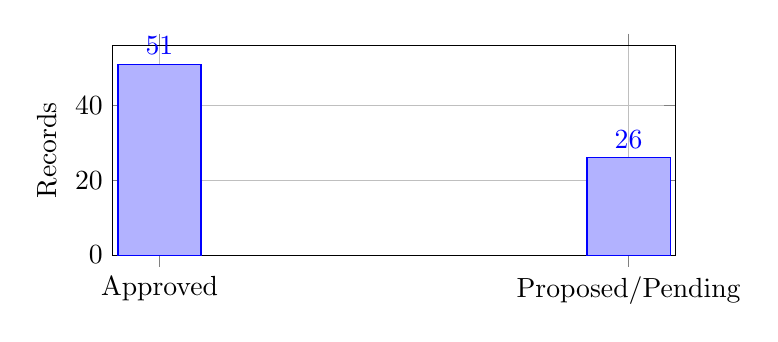
\begin{tikzpicture}
\begin{axis}[
    ybar,
    bar width=30pt,
    width=0.72\textwidth,
    height=0.35\textwidth,
    ylabel={Records},
    symbolic x coords={Approved,Proposed/Pending},
    xtick=data,
    ymin=0,
    nodes near coords,
    nodes near coords align={vertical},
    grid=major
]
\addplot coordinates {(Approved,51) (Proposed/Pending,26)};
\end{axis}
\end{tikzpicture}
\caption{DELTa status distribution from the public update.}
\label{fig:status}
\end{figure}

Figure~\ref{fig:regions} summarizes ISO or RTO linkage for dashboard regions.

\begin{figure}[ht]
\centering
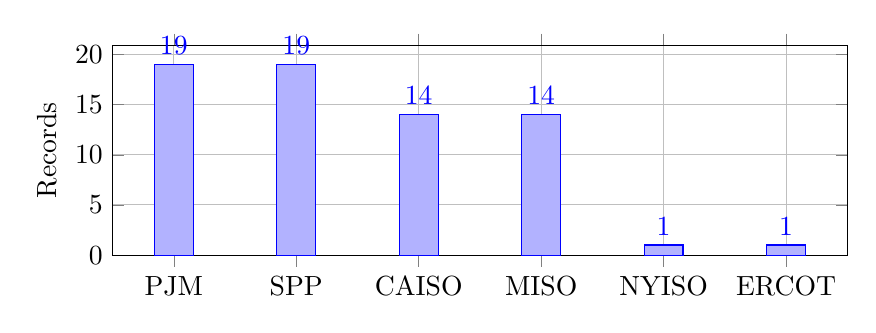
\begin{tikzpicture}
\begin{axis}[
    ybar,
    bar width=14pt,
    width=0.9\textwidth,
    height=0.35\textwidth,
    ylabel={Records},
    symbolic x coords={PJM,SPP,CAISO,MISO,NYISO,ERCOT},
    xtick=data,
    ymin=0,
    nodes near coords,
    grid=major
]
\addplot coordinates {(PJM,19) (SPP,19) (CAISO,14) (MISO,14) (NYISO,1) (ERCOT,1)};
\end{axis}
\end{tikzpicture}
\caption{Coverage of DELTa entries mapped to dashboard market regions.}
\label{fig:regions}
\end{figure}

Minimum-demand thresholds are right-skewed toward large projects (Figure~\ref{fig:hist}).

\begin{figure}[ht]
\centering
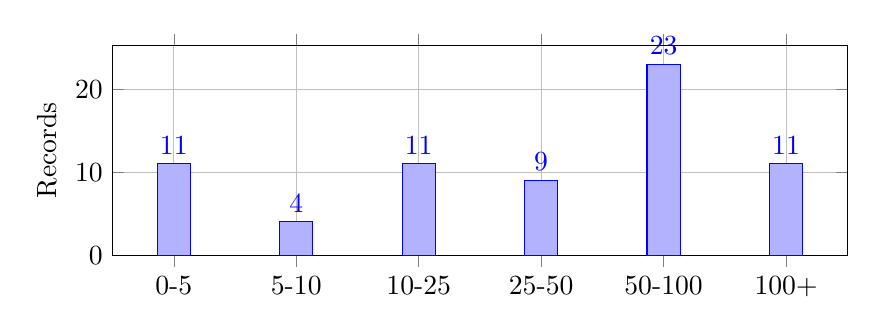
\begin{tikzpicture}
\begin{axis}[
    ybar,
    bar width=12pt,
    width=0.9\textwidth,
    height=0.35\textwidth,
    ylabel={Records},
    symbolic x coords={0-5,5-10,10-25,25-50,50-100,100+},
    xtick=data,
    ymin=0,
    nodes near coords,
    grid=major
]
\addplot coordinates {(0-5,11) (5-10,4) (10-25,11) (25-50,9) (50-100,23) (100+,11)};
\end{axis}
\end{tikzpicture}
\caption{Histogram of minimum demand thresholds (MW) where specified.}
\label{fig:hist}
\end{figure}

\section{System Design}
The service architecture has four stages:
\begin{enumerate}
    \item Ingestion: parse CSV and normalize key fields.
    \item Retrieval: hybrid filtering by structured attributes and semantic chunks.
    \item Generation: constrained JSON response with row-level evidence IDs.
    \item Audit: confidence score and citation validator.
\end{enumerate}

\begin{figure}[ht]
\centering
\begin{tikzpicture}[node distance=10mm, >=latex]
\tikzstyle{box}=[draw, rounded corners, minimum width=25mm, minimum height=9mm, align=center]
\node[box] (ingest) {CSV Ingest\\and Cleaning};
\node[box, right=of ingest] (index) {Hybrid Index\\(fields + text)};
\node[box, right=of index] (retrieval) {Top-k Retrieval\\with Filters};
\node[box, right=of retrieval] (llm) {LLM with\\Schema Guardrails};
\node[box, right=of llm] (output) {Answer +\\Citations};
\draw[->] (ingest) -- (index);
\draw[->] (index) -- (retrieval);
\draw[->] (retrieval) -- (llm);
\draw[->] (llm) -- (output);
\end{tikzpicture}
\caption{DELTa-RAG service architecture.}
\label{fig:architecture}
\end{figure}

\section{Evaluation Plan}
We propose a short benchmark with 50 analyst questions in four categories: policy status lookup, threshold comparison, regional filtering, and narrative extraction. Figure~\ref{fig:eval} illustrates a target quality profile for an initial deployment.

\begin{figure}[ht]
\centering
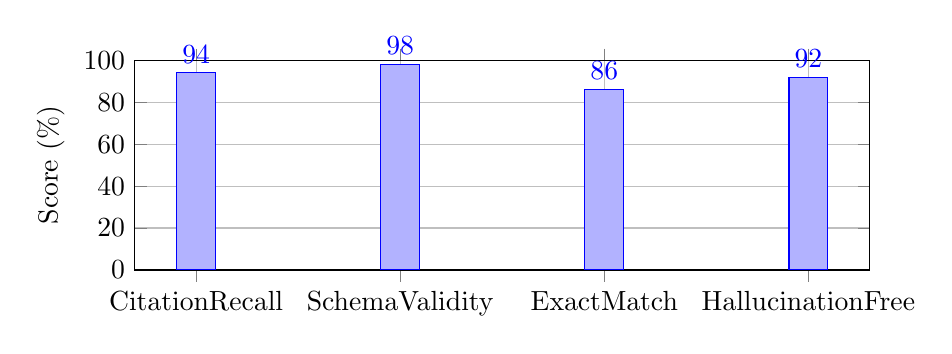
\begin{tikzpicture}
\begin{axis}[
    ybar,
    bar width=14pt,
    width=0.9\textwidth,
    height=0.35\textwidth,
    ylabel={Score (\%)},
    symbolic x coords={CitationRecall,SchemaValidity,ExactMatch,HallucinationFree},
    xtick=data,
    ymin=0, ymax=100,
    nodes near coords,
    grid=major
]
\addplot coordinates {(CitationRecall,94) (SchemaValidity,98) (ExactMatch,86) (HallucinationFree,92)};
\end{axis}
\end{tikzpicture}
\caption{Illustrative target metrics for DELTa-RAG workshop evaluation.}
\label{fig:eval}
\end{figure}

\section{Deployment Notes}
The dashboard can host this service as a policy tab with scope filters (all regions vs selected map region), status filters, and charted summaries. The key engineering constraint is maintaining deterministic field normalization so the model can cite rows precisely.

\section{Conclusion}
DELTa-RAG turns tariff records into a queryable intelligence layer without losing evidence traceability. The approach is practical for policy and market analysts and is a strong candidate for a short conference paper focused on energy informatics and AI for infrastructure decision support.

\section{Target Short-Paper Venues}
Recommended outlets for this LLM paper:
\begin{itemize}
    \item HICSS (Honolulu, Hawaii, USA)
    \item ACM BuildSys Workshops (location varies yearly; often North America or Europe)
    \item ACM e-Energy Workshops (location varies yearly; announced in CFP)
\end{itemize}

\end{document}
